%%%%%%%%%%%%%%%%%%%%%%% file profile.tex %%%%%%%%%%%%%%%%%%%%%%%%%
%
\documentclass[review,12pt,fleqn]{elsarticle}
\usepackage{soul}
\usepackage{xcolor}
% \usepackage{lineno,hyperref}
% \modulolinenumbers[5]

\journal{Journal of \LaTeX\ Templates}

%%%%%%%%%%%%%%%%%%%%%%%
%% Elsevier bibliography styles
%%%%%%%%%%%%%%%%%%%%%%%
%% To change the style, put a % in front of the second line of the current style and
%% remove the % from the second line of the style you would like to use.
%%%%%%%%%%%%%%%%%%%%%%%

%% Numbered
%\bibliographystyle{model1-num-names}

%% Numbered without titles
%\bibliographystyle{model1a-num-names}

%% Harvard
%\bibliographystyle{model2-names.bst}\biboptions{authoryear}

%% Vancouver numbered
%\usepackage{numcompress}\bibliographystyle{model3-num-names}

%% Vancouver name/year
%\usepackage{numcompress}\bibliographystyle{model4-names}\biboptions{authoryear}

%% APA style
%\bibliographystyle{model5-names}\biboptions{authoryear}

%% AMA style
%\usepackage{numcompress}\bibliographystyle{model6-num-names}

%% `Elsevier LaTeX' style
\bibliographystyle{elsarticle-num}
%%%%%%%%%%%%%%%%%%%%%%%


%
% \usepackage{blindtext}
% \usepackage[paperheight=26cm,paperwidth=19cm,margin=0.5cm,heightrounded,showframe]{geometry}

%\smartqed  % flush right qed marks, e.g. at end of proof
%
\usepackage{graphicx}
\usepackage{subfig}
\usepackage{multirow}
\usepackage{hyperref}

\usepackage{amssymb}
\usepackage{amsmath} % Required for some math elements
\usepackage{revsymb} % para fazer o \openone 
% etc.
\usepackage[portuges]{babel}
%
\newcommand{\fim}{ \hfill{\mbox{$\rule{2mm}{2mm}$}}\vskip.6cm }
\newtheorem{teo}{Teorema}
\newtheorem{cor}[teo]{Corolário}
\renewcommand{\appendix}{{\bf Apêndice}}
%%%%%%%%%%%%%%%

\begin{document}
\begin{frontmatter}
\title{Trabalho Computacional de Matemática Discreta 2} 
%  

\author[IPRJ]{Vitor Saraiva de Lima}
\ead{vitorsaraivadelima@gmail.com}

\author[IPRJ]{Mateus Lima Pinho}
\ead{mateuslpinho@gmail.com}

\address[IPRJ]{Curso de Engenharia de Computação,\\
Instituto Politécnico(IPRJ),
\\
Rio de Janeiro State University, 
\\
Rua Bonfim 25, 
  Nova Friburgo, RJ 28625-570, Brazil}
\vskip1cm
\begin{abstract} 
In this work, a program was developed in the SciLab programming language that represents a graph given an adjacency matrix and the coordinates of the points of the same graph, in addition to
demonstrate the dijkstra and search algorithms and the programming of a graphical interface in the last part.
%
\vskip.3cm
%
%
\noindent
{\bf Resumo}
\vskip.3cm
\noindent
Neste trabalho, foi desenvolvido um programa na linguagem de programação SciLab que representa um grafo dada uma matriz adjacência e as coordenadas dos pontos do mesmo grafo, além de 
demonstrar os algorítmos de dijkstra e de busca e a programação de uma interface gráfica na última parte. 
%
\end{abstract}
\vskip.4cm
\begin{keyword}
graph theory \sep matrix adjacency \sep graph algorithms \sep scilab \sep graphical interface
\vskip.2cm
\noindent
{\em Palavras-chave:}
teoria dos grafos \sep matriz adjacência \sep algorítmos de grafos\sep scilab \sep interface gráfica
\end{keyword}
\end{frontmatter}

\section{Introdução}\label{toin}
O trabalho pode ser dividido nas seguintes partes:
\begin{enumerate}
\item \label{item1}Construção de um código-fonte em Scilab implementando os algoritmos de dijkstra e de busca profundidade ou de nível;
\item \label{item2}Construção de um código-fonte em Scilab que dada uma matriz de um grafo produza a matriz adjacência do mesmo, o vetro de arestas e uma matriz B relacionada a representação dada como exemplo na Fig.~\ref{fig1}. Também fazer o processo de volta da matriz B para a matriz adjacência A;
\item \label{item3}Fornecer a matriz de adjacência de um mapa do Brasil, bem como vetores x e y contendo posições de pontos representativos dos estados(não envolve programação);
\item \label{item4}Construção de um código-fonte em Scilab em que dada uma matriz de adjacência, A, e vetores posição de nós, representar na tela do computador o grafo resultante através de uma imagem;
\item \label{item5}Construção de um código-fonte em Scilab que da a opção escolha de mapas (Brasil, Inglaterra, Mercosul) em um menu e cria uma figura dividida em 4 zonas: 
	\begin{enumerate}
	\item \label{item5.1}o mapa da região escolhida;
	\item \label{item5.2}o grafo da região com os nós numerados;
	\item \label{item5.3}o grafo rotulado com os nomes das regiões representadas pelos nós;
	\item \label{item5.4}o grafo com os nós numerados sobreposto ao mapa da região.
	\end{enumerate}
\end{enumerate}

\begin{figure}[!htb]
\centering
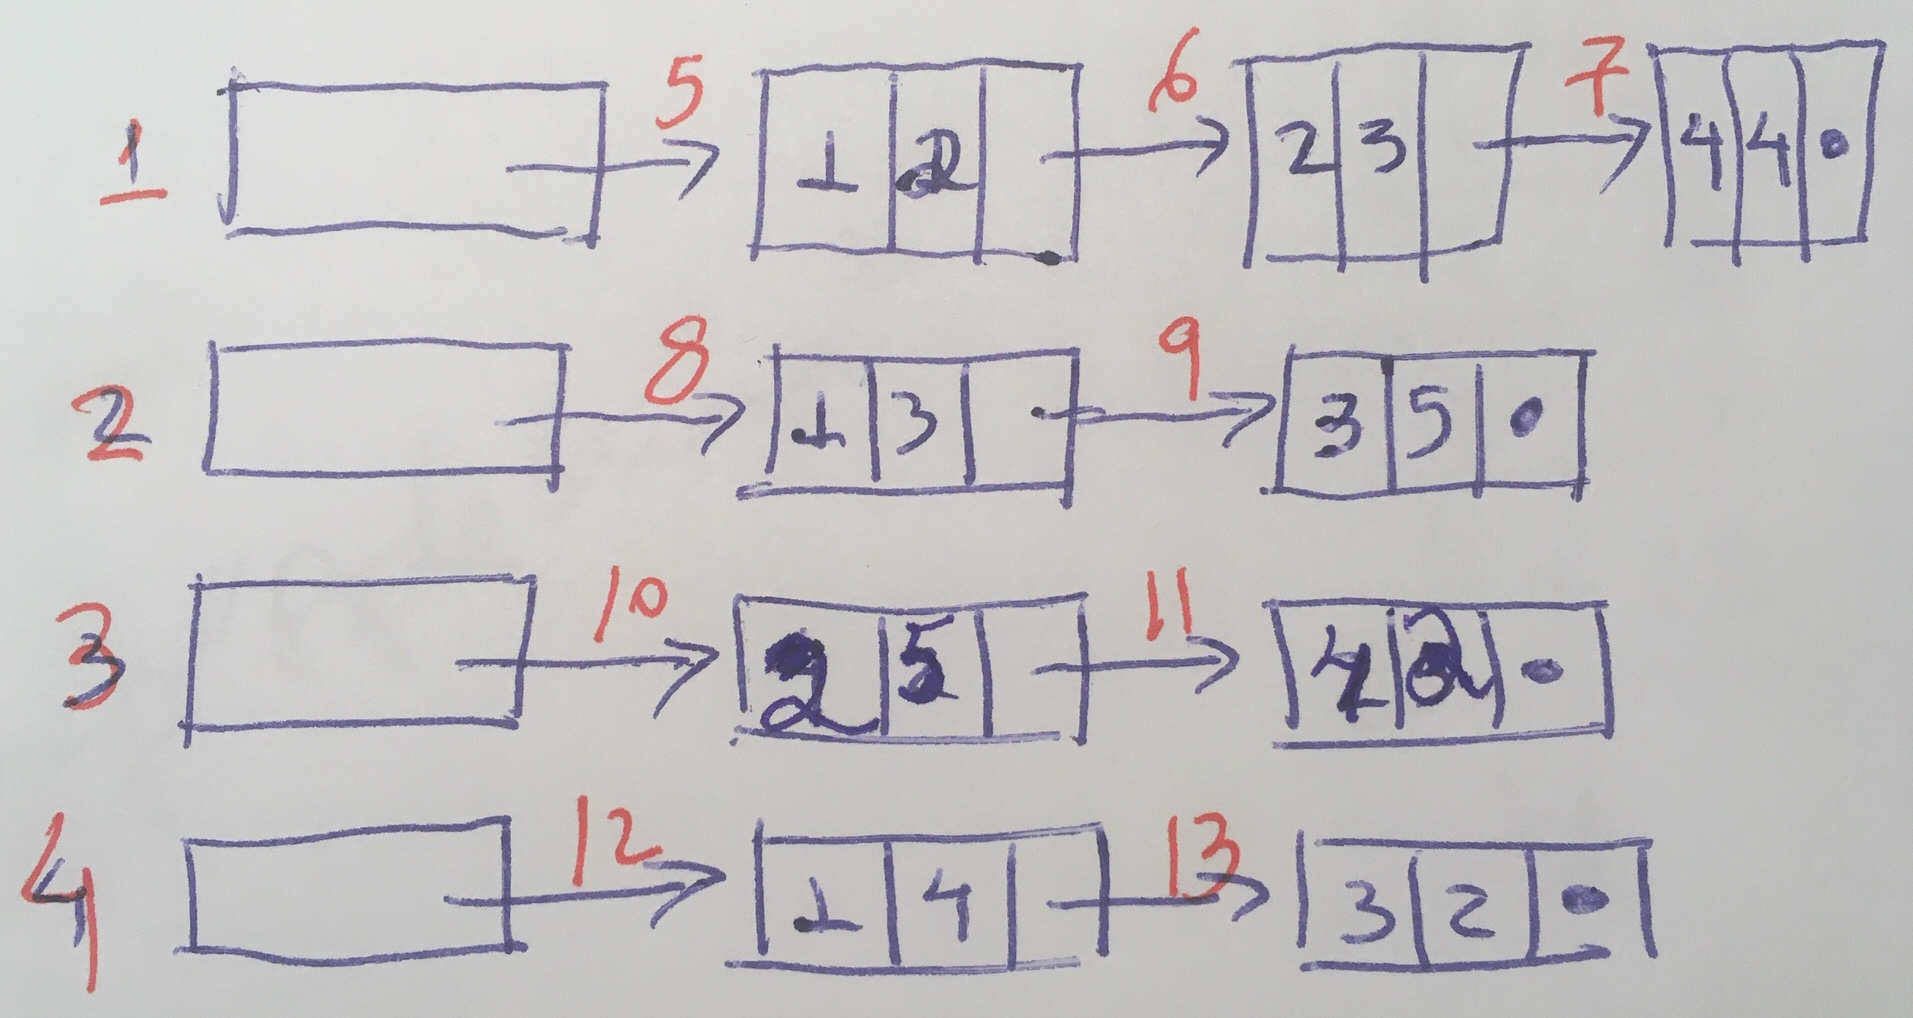
\includegraphics[width=0.72\textwidth]{figura.png}
%
\caption{Exemplo de representação para a matriz B}
\label{fig1}
\end{figure}

\newpage
\section{Algorítmos de dijkstra e de busca}\label{algoritmos}
Nesta seção será abordado o assunto do item \ref{item1} da seção \ref{toin}.
\subsection{Algorítmo de dijkstra} \label{dijkstra}
O algorítmo de dijkstra soluciona o problema do caminho mais curto num grafo dirigido ou não dirigido com arestas de peso não negativo, ele considera um conjunto S de menores caminhos, iniciado com um vértice inicial I e a cada passo do algoritmo busca-se nas adjacências dos vértices pertencentes a S aquele vértice com menor distância relativa a I e adiciona-o a S e, então, repetindo os passos até que todos os vértices alcançáveis por I estejam em S (arestas que ligam vértices já pertencentes a S são desconsideradas).

Um exemplo prático do problema que pode ser resolvido pelo algoritmo de Dijkstra é: alguém precisa se deslocar de uma cidade para outra. Para isso, ela dispõe de várias estradas, que passam por diversas cidades. Qual delas oferece uma trajetória de menor caminho?

O código de scilab começa com o usuário definindo a matriz referente ao grafo:
\[G = \begin{pmatrix}
2 & 3 & \%inf & 4\\ 
3 & 0 & 5 & \%inf\\ 
\%inf & 5 & 0 & 2\\ 
4 & \%inf & 2 & 0
\end{pmatrix}\]

\begin{figure}[!h]
\centering
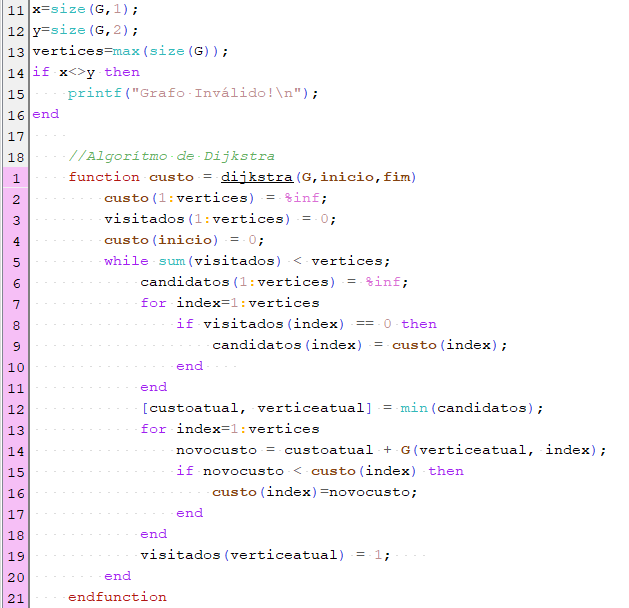
\includegraphics[width=0.72\textwidth]{figura2.png}
%
\caption{Algorítmo de dijkstra scilab}
\label{fig2}
\end{figure}

Onde \%inf representam os nós que não estão conectados entre si. Com base nesse grafo temos a função em scilab demonstrada na Fig.~\ref{fig2}

Este código varre os caminhos possíveis entre o nó início e o nó fim e marca como 1 os nós visitados e 0 os nós não visitados e enquanto percorre os caminhos faz uma comparação para saber qual o caminho de menor custo, sendo o custo representado pelos números na matriz. Os nós início e fim utilizados na função sao gerados aleatoriamente utilizando os seguintes comandos:

\begin{figure}[!h]
\centering
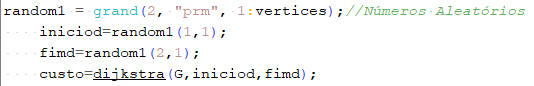
\includegraphics[width=0.72\textwidth]{figura3.png}
%
\caption{Números aleatórios}
\label{fig3}
\end{figure}

Onde random1 é uma matriz 2x4 em que 2 representa a quantidade de números aleatórios nescessários e 4 representa a quantidade de nós, os números a seres selecionados aleatoriamente.

\subsection{Algorítmo de busca em profundidade} \label{busca}
Na teoria dos grafos, busca em profundidade (ou busca em profundidade-primeiro, também conhecido em inglês por Depth-First Search - DFS) é um algoritmo usado para realizar uma busca ou travessia numa árvore, estrutura de árvore ou grafo. Intuitivamente, o algoritmo começa num nó raiz (selecionando algum nó como sendo o raiz, no caso de um grafo) e explora tanto quanto possível cada um dos seus ramos, antes de retroceder(backtracking).


\begin{figure}[!h]
\centering
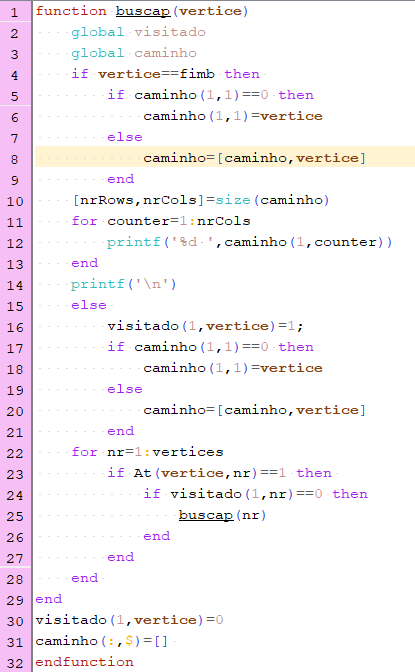
\includegraphics[width=0.5\textwidth]{figura4.png}
%
\caption{Agorítmo de busca em profundidade}
\label{fig4}
\end{figure}

O algoríitmo de busca escolhido foi o de busca em profundidade e ele segue o principio citado em \ref{dijkstra} em que marca 1 os nós visitados e 0 como os não visitados e prossegue até que todos os nós tenham sido listados. O método de varredura segue o mesmo princípiode \ref{dijkstra} em que tem-se um nó inicio e um nó fim que são gerados aleatoriamente com o mesmo método ultilizado na Fig.~\ref{fig3}, demonstrado na Fig.~\ref{fig4} a seguir:


\newpage
\section{Matriz Adjacência} \label{matrizA}
Nesta seção será abordado o assunto do item \ref{item2} da seção \ref{toin}.

O código pega a matriz do grafo mencionada em \ref{dijkstra} e a transforma em uma matriz adjacência, uma matriz de 1's e 0's que representa um grafo, a matriz foi montada simplesmente percorrendo a matriz G e analisando que se A(i,j) fosse zero ou \%inf na matriz A seria 0 e se fosse um número diferente de zero e \%inf seria 1. Após isso foi montado o vetor de arestas simplesmente utilizando o comando "a=sum(At,'r');" que faz a soma das linhas e salva em uma nova matriz  chamada "a".

\begin{figure}[!h]
\centering
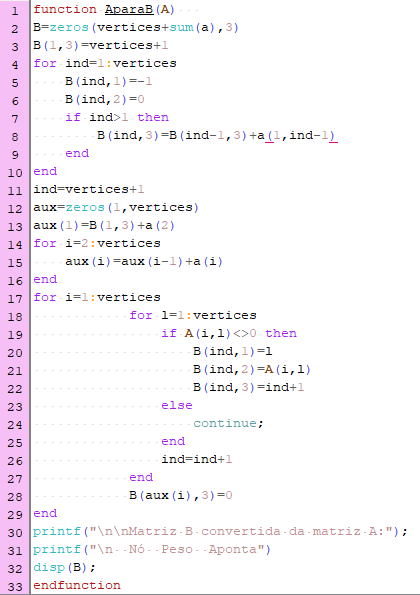
\includegraphics[width=0.7\textwidth]{figura5.png}
%
\caption{Código de transformação da matriz adjacência A para a matriz B}
\label{fig5}
\end{figure}

Após isso a próxima parte do código preecheria a matriz B na coluna "nó" com -1  e com zero na coluna "peso" até a linha que tem mesmo número da quantidade de vértices do grafo. O código também analisa as adjacências dos vértices e completa a matriz B de acordo apontando sempre à linha seguinte a não ser que o número do vértice tenha mudado, demonstrado  no código da Fig.~\ref{fig5}.

A função pega uma dada matriz A e a converte para a matriz B, gerando a matriz a seguir:

\[B = 
\begin{pmatrix}
N\acute{o} & Peso & Aponta\\ 
-1 & 0 & 5\\ 
-1 & 0 & 8\\ 
-1 & 0 & 10\\ 
-1 & 0 & 12\\ 
1 & 2 & 6\\ 
2 & 3 & 7\\ 
4 & 4 & 0\\ 
1 & 3 & 9\\ 
3 & 5 & 0\\ 
2 & 5 & 11\\ 
4 & 2 & 0\\ 
1 & 4 & 13\\ 
3 & 2 & 0
\end{pmatrix}\]

\begin{figure}[!h]
\centering
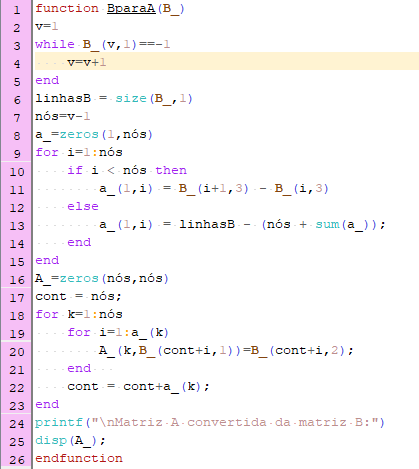
\includegraphics[width=0.7\textwidth]{figura6.png}
%
\caption{Código de transformação da matriz B para a matriz adjacência A}
\label{fig6}
\end{figure}

Foi feito também uma outra função com objetivo oposto à anterior, esta outra função recebe uma matriz B e a transforma em uma matriz adjacência A, código demonstrado na Fig.~\ref{fig6} a seguir:

\section{Matriz adjacência e vetores posição de um mapa do Brasil} \label{mapaBrasil}
\begin{figure}[!h]
\centering
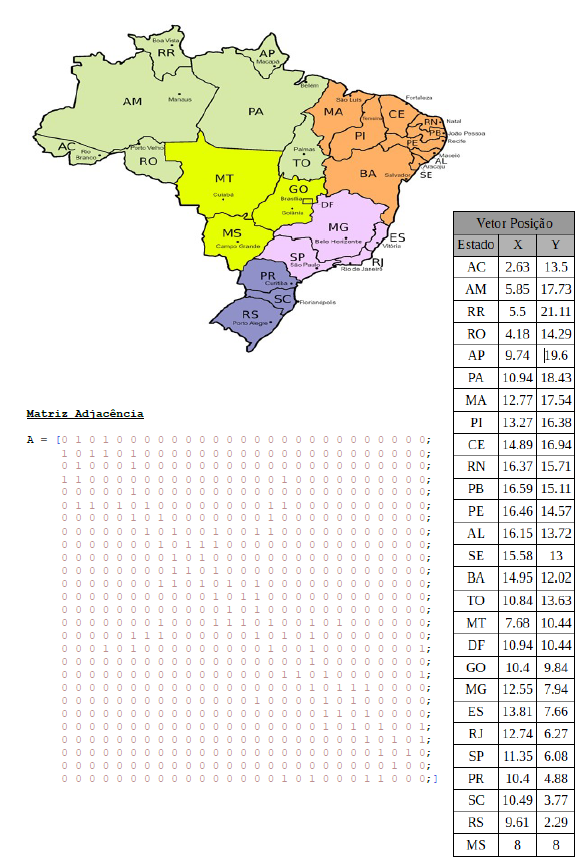
\includegraphics[width=0.8\textwidth]{figura7.png}
%
\caption{Matriz adjacência e tabela de posições de um mapa do Brasil}
\label{fig7}
\end{figure}

Nesta seção será abordado o assunto do item \ref{item3} da seção \ref{toin}. Na Fig.~\ref{fig7} temos uma imagem com o mapa do Brasil dado para o trabalho juntamente com uma matriz adjacência e uma tabela das posições de x e y de seus pontos, que foram gerados utilizando o programa GeoGebra.

\newpage
\section{Montagem de grafo utilizando matriz adjacência e vetor posição} \label{grafo}
Nesta seção será abordado o assunto do item \ref{item4} da seção \ref{toin}. 

\begin{figure}[!htb]
\centering
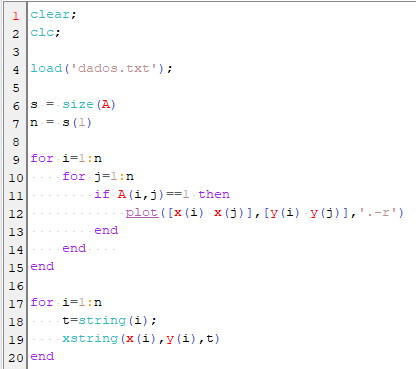
\includegraphics[width=0.7\textwidth]{figura8.png}
%
\caption{Código-fonte da montagem de grafos}
\label{fig8}
\end{figure}

Nesta parte foi feito um código  mostrado na  Fig.~\ref{fig8} que tendo uma matriz adjacência de um grafo e dois vetores de posição, um de x e um de y, monta um grafo em forma de imagem.

\section{Menu iterativo} \label{menu}
Nesta seção será abordado o assunto do item \ref{item5} da seção \ref{toin}. Nesse item do trabalho foi utilizada a ferramenta GuiBuilder do scilab, que permite criar uma interface garffica visualmente e depois gerar o código.

\begin{figure}[!htb]
\centering
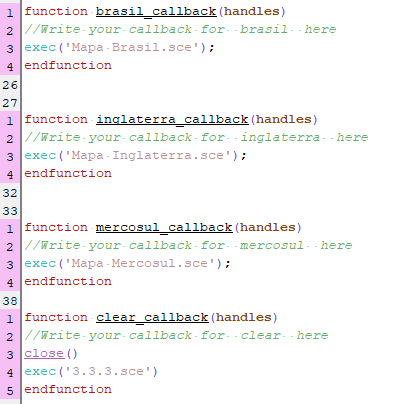
\includegraphics[width=0.7\textwidth]{figura9.png}
%
\caption{Código-fonte da interface gráfica}
\label{fig9}
\end{figure}

\newpage
Foi criada uma interface simples com quatro botões: um três para selecionar Brasil, Inglaterra ou Mercosul e um para limpar o que foi gerado. No código desse programa foi programado para que quando pressionado um dos botões das opções chama-se um outro código de scilab que geraria a imagem da opção selecionada como mostra a Fig.~\ref{fig9}

O código que gera a imagem dos mapas com os seus grafos equivalentes citados em \ref{item5.1},\ref{item5.2},\ref{item5.3} e \ref{item5.4} da seção \ref{toin} tem o mesmo código mudando somente o nomes dos arquivos de imagem dos mapa e do de dados, na Fig.~\ref{fig10} a seguir está o código citado.


\begin{figure}[!htb]
\centering
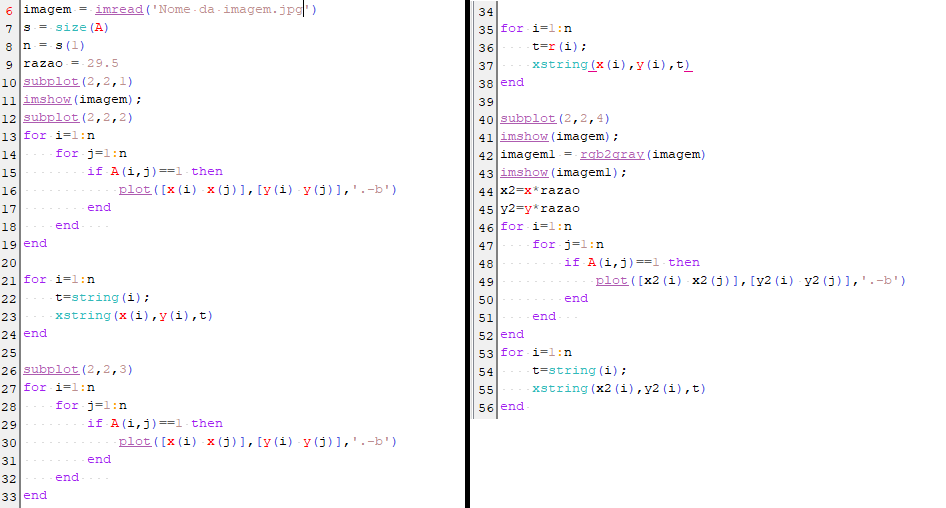
\includegraphics[width=1\textwidth]{figura10.png}
%
\caption{Código-fonte da montagem dos mapas}
\label{fig10}
\end{figure}

\newpage
Nas Fig.~\ref{fig11}, \ref{fig12} e \ref{fig13} a seguir estão os mapas gerados pelo programa.

\begin{figure}[!htb]
\centering
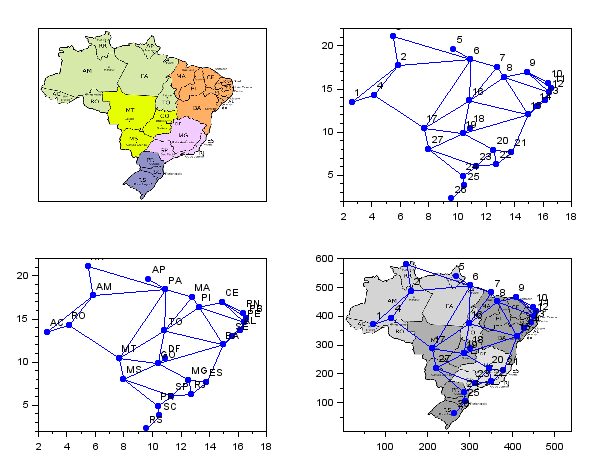
\includegraphics[width=0.7\textwidth]{figura11.png}
%
\caption{Mapa Brasil}
\label{fig11}
\end{figure}

\begin{figure}[!htb]
\centering
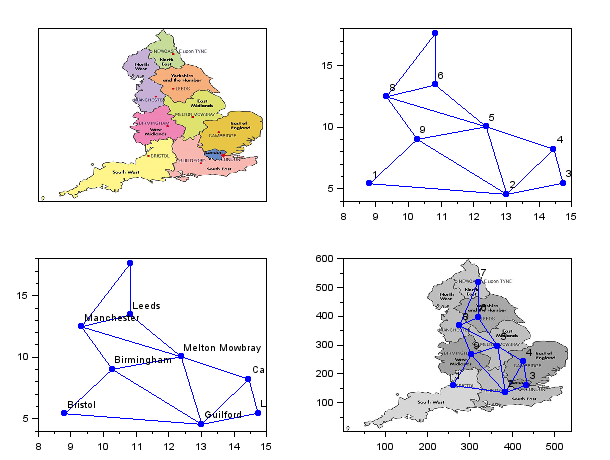
\includegraphics[width=0.7\textwidth]{figura12.png}
%
\caption{Mapa Inglaterra}
\label{fig12}
\end{figure}

\begin{figure}[!htb]
\centering
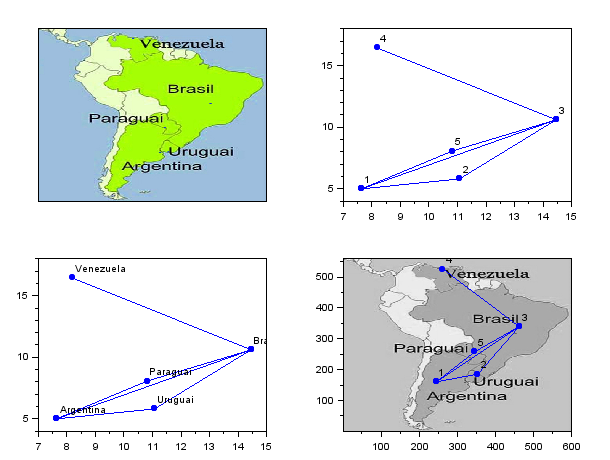
\includegraphics[width=0.7\textwidth]{figura13.png}
%
\caption{Mapa Mercosul}
\label{fig13}
\end{figure}

\newpage
\section{Conclusão}
Foi concluído que este trabalho computacional foi algo bom a ser feito, pois ajudou a adcionar conhecimentos anteriormente não possuídos, como o conhecimento da linguagem de programação SciLab, que é muito boa para programas envolvendo cálculos matemáticos por sua grande variedade de funções trantando tal assunto e por ser próxima da linguagem de MatLab que é outra linguagem ótima para o mesmo, juntamente com o novo conhecimento adquirido de interfaces gráficas.

Uma das grandes dificuldades encontradas para o desenvolvimento do trabalho foi a falta de conhecimento da linguagem, por ser algo que nunca foi visto por nossa parte e por consequência disso uma dificuldade na implementação das tarefas solicitadas para o trabalho.

\begin{thebibliography}{}
\footnotesize
\bibitem{gersting2007}Judith L. Gersting, (2007)  {\em Mathematical structures for computer science}, Macmillan

\bibitem{costa2011}Polyanna Possani da Costa, (2011) {\em Teoria dos grafos e suas aplica{\c{c}}{\~o}es}, Universidade Estadual Paulista (UNESP)

\bibitem{cormen2002} Thomas H. Cormen and Charles E. Leiserson and Ronald L. Rivest and Clifford Stein, (2002) {\em Algoritmos: teoria e pr{\'a}tica}, Editora Campus, Vol. 2

\bibitem{1}\url{https://help.scilab.org/docs/5.4.1/pt_BR/index.html} 

\bibitem{2}\url{https://www.scilab.org/tutorials/application-development-\%E2\%80\%93-gui-building} 

\bibitem{3}\url{https://rosettacode.org/wiki/Dijkstra\%27s_algorithm}

\bibitem{4}\url{https://www.ime.usp.br/~pf/algoritmos_para_grafos/aulas/dfs.html}
\end{thebibliography}
%\include{texto_body_ARn}
%\include{texto_conc}
%\include{ref_bib}
%\include{texto_supp}
\end{document}
